\documentclass[a4paper,11pt]{exam}
%\printanswers % pour imprimer les réponses (corrigé)
\noprintanswers % Pour ne pas imprimer les réponses (énoncé)
\addpoints % Pour compter les points
% \noaddpoints % pour ne pas compter les points
%\qformat{\textbf{\thequestion ) } }
%\qformat{\textbf{\thequestion )} (\thepoints) \\} % Pour définir le style des questions (facultatif)
\usepackage{color} % définit une nouvelle couleur
\shadedsolutions % définit le style des réponses
% \framedsolutions % définit le style des réponses
\definecolor{SolutionColor}{rgb}{0.8,0.9,1} % bleu ciel
\renewcommand{\solutiontitle}{\noindent\textbf{Solution:}\par\noindent} % Définit le titre des solutions




\makeatletter

\def\maketitle{{\centering%
	\par{\huge\textbf{\@title}}%
	\par{\@date}%
	\par}}

\makeatother

\lhead{NOM Pr\'enom :}
\rhead{\textbf{Les r\'eponses doivent \^etre justifi\'ees}}
\cfoot{\thepage / \pageref{LastPage}}


%\usepackage{../../pas-math}
%\usepackage{../../moncours}


%\usepackage{pas-cours}
%-------------------------------------------------------------------------------
%          -Packages nécessaires pour écrire en Français et en UTF8-
%-------------------------------------------------------------------------------
\usepackage[utf8]{inputenc}
\usepackage[frenchb]{babel}
\usepackage[T1]{fontenc}
\usepackage{lmodern}
\usepackage{textcomp}



%-------------------------------------------------------------------------------

%-------------------------------------------------------------------------------
%                          -Outils de mise en forme-
%-------------------------------------------------------------------------------
\usepackage{hyperref}
\hypersetup{pdfstartview=XYZ}
%\usepackage{enumerate}
\usepackage{graphicx}
\usepackage{multicol}
\usepackage{tabularx}
\usepackage{multirow}


\usepackage{anysize} %%pour pouvoir mettre les marges qu'on veut
%\marginsize{2.5cm}{2.5cm}{2.5cm}{2.5cm}

\usepackage{indentfirst} %%pour que les premier paragraphes soient aussi indentés
\usepackage{verbatim}
\usepackage{enumitem}
\usepackage[usenames,dvipsnames,svgnames,table]{xcolor}

\usepackage{variations}

%-------------------------------------------------------------------------------


%-------------------------------------------------------------------------------
%                  -Nécessaires pour écrire des mathématiques-
%-------------------------------------------------------------------------------
\usepackage{amsfonts}
\usepackage{amssymb}
\usepackage{amsmath}
\usepackage{amsthm}
\usepackage{tikz}
\usepackage{xlop}
%-------------------------------------------------------------------------------



%-------------------------------------------------------------------------------


%-------------------------------------------------------------------------------
%                    - Mise en forme avancée
%-------------------------------------------------------------------------------

\usepackage{ifthen}
\usepackage{ifmtarg}


\newcommand{\ifTrue}[2]{\ifthenelse{\equal{#1}{true}}{#2}{$\qquad \qquad$}}

%-------------------------------------------------------------------------------

%-------------------------------------------------------------------------------
%                     -Mise en forme d'exercices-
%-------------------------------------------------------------------------------
%\newtheoremstyle{exostyle}
%{\topsep}% espace avant
%{\topsep}% espace apres
%{}% Police utilisee par le style de thm
%{}% Indentation (vide = aucune, \parindent = indentation paragraphe)
%{\bfseries}% Police du titre de thm
%{.}% Signe de ponctuation apres le titre du thm
%{ }% Espace apres le titre du thm (\newline = linebreak)
%{\thmname{#1}\thmnumber{ #2}\thmnote{. \normalfont{\textit{#3}}}}% composants du titre du thm : \thmname = nom du thm, \thmnumber = numéro du thm, \thmnote = sous-titre du thm

%\theoremstyle{exostyle}
%\newtheorem{exercice}{Exercice}
%
%\newenvironment{questions}{
%\begin{enumerate}[\hspace{12pt}\bfseries\itshape a.]}{\end{enumerate}
%} %mettre un 1 à la place du a si on veut des numéros au lieu de lettres pour les questions 
%-------------------------------------------------------------------------------

%-------------------------------------------------------------------------------
%                    - Mise en forme de tableaux -
%-------------------------------------------------------------------------------

\renewcommand{\arraystretch}{1.7}

\setlength{\tabcolsep}{1.2cm}

%-------------------------------------------------------------------------------



%-------------------------------------------------------------------------------
%                    - Racourcis d'écriture -
%-------------------------------------------------------------------------------

% Angles orientés (couples de vecteurs)
\newcommand{\aopp}[2]{(\vec{#1}, \vec{#2})} %Les deuc vecteurs sont positifs
\newcommand{\aopn}[2]{(\vec{#1}, -\vec{#2})} %Le second vecteur est négatif
\newcommand{\aonp}[2]{(-\vec{#1}, \vec{#2})} %Le premier vecteur est négatif
\newcommand{\aonn}[2]{(-\vec{#1}, -\vec{#2})} %Les deux vecteurs sont négatifs

%Ensembles mathématiques
\newcommand{\naturels}{\mathbb{N}} %Nombres naturels
\newcommand{\relatifs}{\mathbb{Z}} %Nombres relatifs
\newcommand{\rationnels}{\mathbb{Q}} %Nombres rationnels
\newcommand{\reels}{\mathbb{R}} %Nombres réels
\newcommand{\complexes}{\mathbb{C}} %Nombres complexes


%Intégration des parenthèses aux cosinus
\newcommand{\cosP}[1]{\cos\left(#1\right)}
\newcommand{\sinP}[1]{\sin\left(#1\right)}


%Probas stats
\newcommand{\stat}{statistique}
\newcommand{\stats}{statistiques}
%-------------------------------------------------------------------------------

%-------------------------------------------------------------------------------
%                    - Mise en page -
%-------------------------------------------------------------------------------

\newcommand{\twoCol}[1]{\begin{multicols}{2}#1\end{multicols}}


\setenumerate[1]{font=\bfseries,label=\textit{\alph*})}
\setenumerate[2]{font=\bfseries,label=\arabic*)}


%-------------------------------------------------------------------------------
%                    - Elements cours -
%-------------------------------------------------------------------------------





%\usepackage{fullpage}
\author{\ }
\date{8 Octobre 2019}
\title{$6^e C$ : DS num\'ero 1}


\begin{document}
%	\usepackage{fancyhdr}
%	
%	\pagestyle{fancy}
%	\fancyhf{}
	%\rhead{Share\LaTeX}

	\maketitle
	
\begin{center}
	\textbf{Calculatrice interdite, le soin et la qualité de la rédaction seront pris en compte}
\end{center}

\begin{small}
	\begin{center}
		\begin{tabular}{|@{\ }l@{\ }|@{\ }c@{\ }|@{\ }c@{\ }|@{\ }c@{\ }|@{\ }c@{\ }|}
			\hline
			\textbf{Compétence} & \textbf{MI} & \textbf{MF} & \textbf{MS} & \textbf{TBM} \\
			\hline
			\textbf{Représenter} (Différentes écritures d'un même nombre : fractions/décimaux. ) &  \ \ & \ \ & \ \ & \ \  \\
			\hline	
			\textbf{Modéliser} (Résolution de problèmes de la vie courante.) & \ \ & \ \ &  \ \  & \ \ \\
			\hline
			%			 \textbf{Communiquer} (Expliquer sa démarche, son raisonnement ) &  \ \ & \ \ & \ \ & \ \  \\
			%			\hline
		\end{tabular}
	\end{center}
\end{small}	

	
	
	

%\newpage

\section{Identifier un nombre (2 points)}

Je suis un nombre décimal :
\begin{itemize}
	\item Ma partie entière est égale à la somme (l'addition) des chiffres de la partie décimale de \num{62.378};
	\item Mon chiffre des dixièmes est égal à la somme des chiffres de ma partie entière;
	\item Mon chiffre des millièmes est égal au double de mon chiffre des dizaines;
	\item Si j'additionne tous mes chiffres, le résultat est 23.
	
\end{itemize}

\begin{questions}
	\question[2] Qui suis-je ? Donner deux nombres possibles.
	
	\begin{solution}
		\begin{itemize}
			\item Ma partie entière est égale à 18 (3 +  7 + 8);
			\item Mon chiffre des dixièmes est 9 (1 + 8);
			\item Mon chiffre des millièmes est 2;
			\item Je suis \num{18.932} (1+8+9+3+2 = 23), ou \num{18.9221} (1 + 8 + 9 +2 +2 + 1 = 23)
		\end{itemize}
	
	
	\end{solution}
\end{questions}

\section{Combinaison d'un cadenas (4 points)}

%illustration phare 80 page 24

Marie à oublié la combinaison de son cadenas à 3 chiffres. Elle se souvient seulement que cette combinaison est composée des chiffres 8 ; 5 et 0.

\begin{questions}
	\question[2] \'Ecrire toutes les combinaisons possibles.
	\question[2] \'Ecrire en toutes lettres chacun des nombres de la question précédente.
\end{questions}

%\begin{myact}{1 Différentes écritures des nombres}
%
%	\label{act:nbres}
%	
%	\begin{enumerate}
%		\item Donner deux nombres à 2, 3, 4 et 5 chiffres.
%		
%		%\item \'Ecrire les nombres suivants en toutes lettres : \num{32}, \num{128} et \num{1024}. 
%		\item \'Ecrire  le nombre 25146041337 en séparant les classes.
%		\item La planète Mars a un rayon d'environ \textbf{3,4 milliers} de km, une superficie d'environ \textbf{144,8 millions} de $km^2$ et un volume d'environ \textbf{163 milliards} de $km^3$.
%		
%		\'Ecrire les trois nombres en gras en utilisant que des chiffres.
%		
%		\item Lire le texte ci-dessous, puis écrire en chiffres les nombres en gras.
%		
%			\begin{center}
%				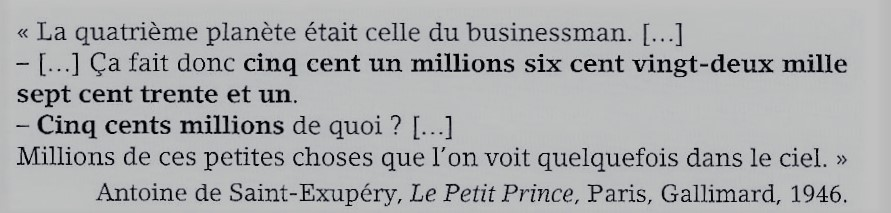
\includegraphics[scale=1.1]{img/act1}
%			\end{center}
%	\end{enumerate}
%\end{myact}

%\begin{myactrep}{1 Différentes écritures des nombres}
	
%	\begin{enumerate}
%		\item 
%			\begin{itemize}
%				\item 17 et 42 sont des nombres à 2 chiffres;
%				\item 128 et 512 sont des nombres à 3 chiffres;
%				\item \num{2048} et \num{4096} sont des nombres à 4 chiffres;
%				\item \num{16384} et \num{65536} sont des nombres à 5 chiffres.
%			\end{itemize}
%		
%		%\item \'Ecrire les nombres suivants en toutes lettres : \num{32}, \num{128} et \num{1024}. 
%		\item Le nombre 25146041337 s'écrit \num{25146041337}.
%		\item 
%			\begin{itemize}
%				\item 3,4 milliers s'écrit \num{3400};
%				\item 144,8 millions s'écrit \num{144800000};
%				\item 163 milliards s'écrit \num{163000000000}.
%			\end{itemize}
%		
%		\item .
%			\begin{itemize}
%				\item Cinq-cent-un-millions-six-cent-vingt-deux-mille-sept-cent trente-et-un s'écrit \num{501622731};
%				\item Cinq-cent-millions s'écrit \num{500000000}.
%			\end{itemize}
%
%	\end{enumerate}
%\end{myactrep}


\begin{mydef}
	\begin{itemize}
		\item Il existe 10 \kw{chiffres} : 
		\iftoggle{eleve}{%
			\iftoggle{dys}{%
				0, 1, 2, 3, 4, 5, 6, 7, 8 et 9.	
			}{
		}
		}{%
			0, 1, 2, 3, 4, 5, 6, 7, 8 et 9.	
		}
		
		\item On utilise les chiffres pour  
		\iftoggle{eleve}{%
			\iftoggle{dys}{%
				écrire des	nombres
			}{
			}
		}{%
			écrire des nombres
		}.
		
		
	\end{itemize}
\end{mydef}

\begin{myexs}
	\begin{enumerate}
		\item Quels nombres peut-on écrire avec les chiffres  2 et 4 ?
		
		\iftoggle{eleve}{%
			\iftoggle{dys}{%
				On peut écrire les nombres 
			}{
				\vspace*{0.5cm}
			}
		}{%
			On peut écrire les nombres 24 et 42.
		}
		
		\item Le nombre \num{49096} s'écrit avec quels chiffres ? 
		
		\iftoggle{eleve}{%
			\iftoggle{dys}{%
				Il s'écrit avec les chiffres 4, 0, 9 et 6.
			}{
				\vspace*{0.5cm}
			}
		}{%
			Il s'écrit avec les chiffres 4, 0, 9 et 6.
		}
		
		
	\end{enumerate}
\end{myexs}





\begin{mydefs}
	\begin{itemize}
		\item Pour mieux lire un grand nombre, on regroupe \iftoggle{eleve}{%
			\iftoggle{dys}{%
				 ses chiffres en classes par groupe de 3.
			}{
				\vspace*{0.75cm}
			}
		}{%
			 ses chiffres en classes par groupe de 3.
		}
		
		\item Un \kw{nombre décimal} possède \iftoggle{eleve}{%
			\iftoggle{dys}{%
				une \kw{partie entière} (avant la virgule) et une \kw{partie décimale} (après la virgule).
			}{
				\vspace*{0.75cm}
			}
		}{%
			une \kw{partie entière} (avant la virgule) et une \kw{partie décimale} (après la virgule).
		}
		
		\item Un \kw{nombre entier} est un nombre décimal où 
		\iftoggle{eleve}{%
			\iftoggle{dys}{%
				 la partie décimale ne contient que des zéros. Dans ce cas la partie décimale n'apparait pas.
			}{
				\vspace*{0.75cm}\\
				Dans ce cas la partie décimale n'apparait pas.
			}
		}{%
			 la partie décimale ne contient que des zéros. Dans ce cas la partie décimale n'apparait pas.
		} 
		
	\end{itemize}
\end{mydefs}

\begin{center}
	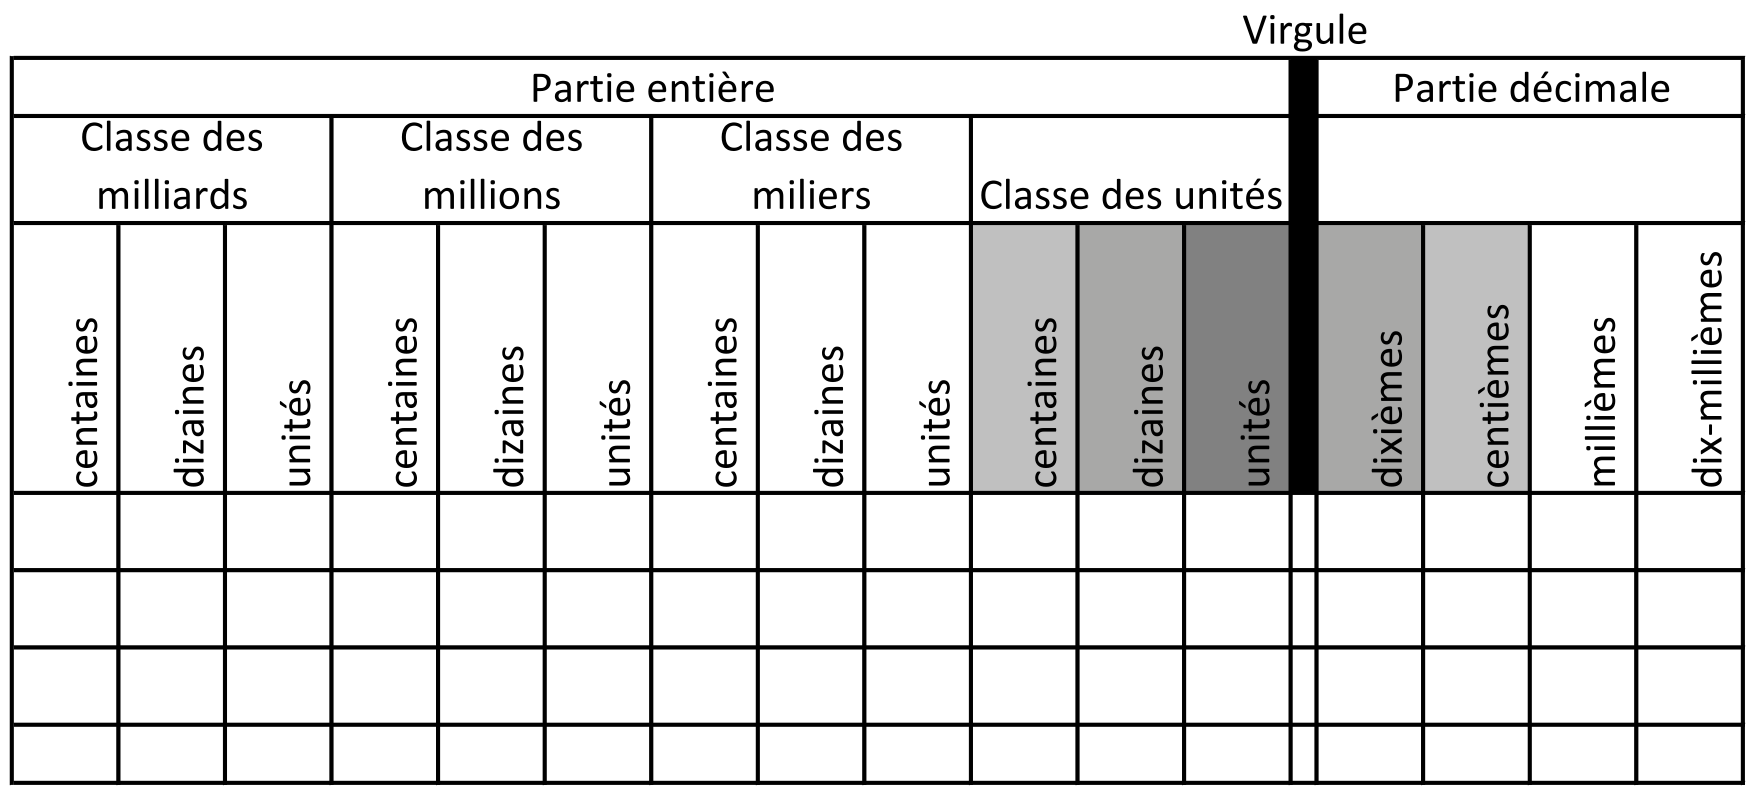
\includegraphics[scale=0.34]{img/tab_rangs}
\end{center}

\begin{myexs}
	\begin{enumerate}
		\item \'Ecrire correctement le nombre 1845937126 :
		
		\iftoggle{eleve}{%
			\iftoggle{dys}{%
				Ce nombre s'écrit 
			}{
				\vspace*{1cm} %\ \\
				
			}
		}{%
			Ce nombre s'écrit \num{1845937126}.
		} 
		
		%\item Le nombre \num{2048} est un nombre entier.
		\item Donner la partie entière et la partie décimale de  \num{5239.67} :
		
		\iftoggle{eleve}{%
			\iftoggle{dys}{%
				La partie entière de   \num{5239.67} est \hspace*{3cm} et sa partie décimale est 	
			}{
				\vspace*{1cm} %\ \\
				
			}
		}{%
			La partie entière de   \num{5239.67} est \num{5239} et sa partie décimale est 67.	
		}
	
		
		
		
		
		\item Donner le chiffre des centaines et le nombre de dizaines de \num{1337}.
		
		
		\iftoggle{eleve}{%
			\iftoggle{dys}{%
				Dans \num{1337}, le chiffre des centaines est \hspace*{2cm} et le nombre de dizaines est \hspace*{2cm}.
			}{
				\vspace*{1cm} %\ \\
				
			}
		}{%
			Dans \num{1337}, le chiffre des centaines est 3 et le nombre de dizaines est 133.
		}
		
		
		\item Donner une autre écriture possible du nombre 124 :
		
		\iftoggle{eleve}{%
			\iftoggle{dys}{%
				Le nombre entier \num{124} peut aussi s'écrire 
			}{
				\vspace*{1cm} %\ \\
				
			}
		}{%
			Le nombre entier \num{124} peut aussi s'écrire \num{124.00}.
		}
	

	\end{enumerate}
\end{myexs}


\begin{mymethname}{\'Ecrire un nombre en toutes lettres}
	\begin{itemize}
		\item Tous les mots qui désignent un nombre sont invariables, sauf <<vingt>> et <<cent>>;
		\item Les mots <<milliard>>, <<million>>, <<dixième>> ne désignent pas des nombres, ils prennent un <<s>> au pluriel;
		\item 80 s'écrit <<quatre-vingts>> sauf s'il est suivi d'un autre nombre;
		\item 100 s'écrit <<cents>> s'il est multiplié et non suivi d'un autre nombre, dans les autres cas il ne prend pas de <<s>>;
		\item On écrit un trait d'union entre chaque mot d'un nombre.
	\end{itemize}
\end{mymethname}

\begin{myexs}
	
	\iftoggle{eleve}{%
		\begin{itemize}
			\item 180 s'écrit %\pause <<cent-quatre-vingts>>;\pause
			\item \num{1300} s'écrit %\pause <<mille-trois-cents>>;\pause
			\item \num{4025035} s'écrit %\pause <<quatre-millions-vingt-cinq-mille-trente-cinq>>;
			\item \num{134.25} s'écrit %\pause <<cent-trente-quatre unités vingt-cinq centièmes.
		\end{itemize}
	}{%
		\begin{itemize}
			\item 180 s'écrit \pause <<cent-quatre-vingts>>;\pause
			\item \num{1300} s'écrit \pause <<mille-trois-cents>>;\pause
			\item \num{4025035} s'écrit \pause <<quatre-millions-vingt-cinq-mille-trente-cinq>>;
			\item \num{134.25} s'écrit \pause <<cent-trente-quatre unités vingt-cinq centièmes.
		\end{itemize}
	}
	
\end{myexs}

%\begin{myexos}
%	\begin{itemize}
%		\item Exercices 1 et 2 page 16 : identifier les chiffres d'un rang donné;
%		\item \Exo{4}{16} : décomposition d'un nombre;
%		\item \Exo{7}{16} : \'ecriture décimale d'un nombre donné en toutes lettres;
%		\item Exercices 8 ,9 et 13 page 17 : problèmes identifier des nombres selon des critères donnés.
%		\item \Exo{11}{17} : regroupement des chiffres d'un nombre en classes.
%		\item \Exo{14}{17} : enlever les zéros inutiles.
%	\end{itemize}
%	
%\end{myexos}


\begin{myact}{2 Classement}
	Activité 3 page 13
\end{myact}

\begin{myactrep}{2 Classement}
	\begin{enumerate}
		\item Le colis le plus lourd est celui qui a une masse de \num{15.3} kg et \num{13.999} kg pour le plus léger.
		\item On a donc :
		
		\num{13.999} < \num{14.15} < \num{14.509} < \num{14.575} < \num{14.59} <  \num{14.805} < \num{15.29} < \num{15.3}
	\end{enumerate}
\end{myactrep}

\begin{mydefs}
	\begin{itemize}
		\item \kw{Comparer} des nombres, c'est dire si un est plus petit ou plus grand que l'autre ou s'ils sont égaux.
		
		\item Ranger des nombres du plus petit au plus grand, c'est les classer par \kw{ordre croissant}.
		
		\item Ranger des nombres du plus grand au plus petit, c'est les classer par \kw{ordre décroissant}.
		
		\item \kw{Encadrer} un nombre, c'est trouver un nombre plus petit \textbf{et} un nombre plus grand que ce nombre.
		
		\item \kw{Intercaler} un nombre entre deux autres, c'est un nombre compris entre ces deux nombres.
	\end{itemize}
\end{mydefs}

\begin{myexs}
	\begin{itemize}
		\item 42 < 128, \pause se lit <<42 est inférieur à (ou plus petit que) 128>>;\pause
		\item 1337 < 1024,\pause se lit <<\num{1337} est supérieur à (ou plus grand que) \num{1024}>>;\pause
		\item 2 < \num{3.2} < \num{6.4} < \num{25.6} : ces nombres sont rangés dans l'ordre \pause croissant;\pause
		\item 123 > \num{45.6} > \num{7.89} > \num{5} : ces nombres sont rangés dans l'ordre \pause décroissant;\pause
		\item Encadrement de 21 à l'unité près : \pause 20 < 21 < 22 ;\pause
		\item Encadrement de \num{21.987} au centième près : \pause \num{21.977} < \num{21.987} < \num{21.997} ;\pause
	\end{itemize}
\end{myexs}

\begin{myexos}
	\begin{itemize}
		\item \Exo{16}{18} : Intercaler des nombres;
		\item Exercices 17 et 18 page 18 : Comparer des nombres;
		\item \Exo{19}{18} : Ordre croissant
		\item \Exo{20}{18} : Ordre décroissant
		\item Exercices 23 et 24 page 18 : Encadrer des nombres;
		\item \Exo{25}{19} : Comparer des nombres;
		\item \Exo{26}{19} : Ordre croissant;
		\item \Exo{27}{19} : Ordre décroissant.
	\end{itemize}
\end{myexos}


\begin{myprop}
	Un point placé sur une droite graduée est repéré par un nombre, son \kw{abscisse}.
\end{myprop}

\begin{myex}
	\begin{center}
		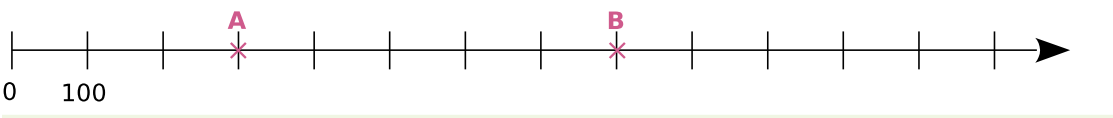
\includegraphics[scale=0.5]{img/axe}
	\end{center}

	\begin{itemize}
		\item L'abscisse du point A est :
		\item L'abscisse du point B est :
		\item L'abscisse du point C est : 500;
		\item L'abscisse du point D est \num{1100}.
	\end{itemize}
\end{myex}



\section{Verre doseur (4 points)}


En cuisine, il peut être pratique d'utiliser un verre doseur. Celui-ci permet de mesurer des masses de farine, de riz, de sucre et un volume de liquide.
Quelle quantité contient ce verre doseur, s'il s'agit :

\begin{center}
	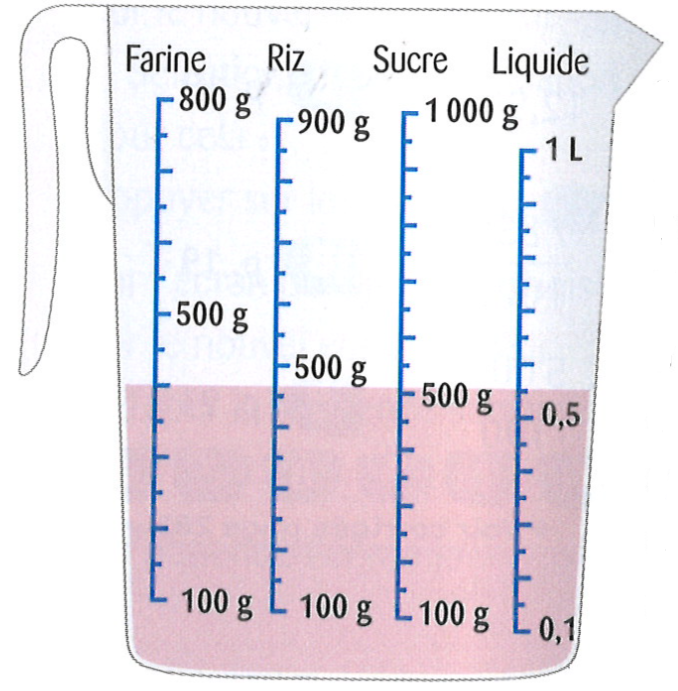
\includegraphics[scale=1]{img/verre}
\end{center}
\begin{questions}
	
	\begin{multicols}{2}
		
	\question[1] 
	
	de farine ? 
	
	
	\question[1]
	
	de riz ?
	
	
	\question[1]
	
	de sucre ? 
	
	
	\question[1]
	
	d'huile ?
	\end{multicols}
	
\end{questions}

%\begin{mydefs}
	Dans un triangle :
	\begin{itemize}
		\item La \kw{médiatrice} d'un coté est la droite perpendiculaire à ce coté et passant par son milieu.
		
		\item Une droite qui passe par un sommet et est perpendiculaire à la droite qui porte le coté opposé est une \kw{hauteur} du triangle. 
	\end{itemize}
\end{mydefs}

\begin{myexs}
	\begin{multicols}{2}
		Dans la figure ci-contre :
		
		\begin{itemize}
			\item $(AH)$ est la hauteur issue de $A$, $H$ est le pied de cette hauteur;
			\item $(BE)$ est la hauteur issue de $B$, $E$ est le pied de cette hauteur;
			\item $(DF)$ est la médiatrice du coté $[BC]$;
		\end{itemize}
		\begin{center}
			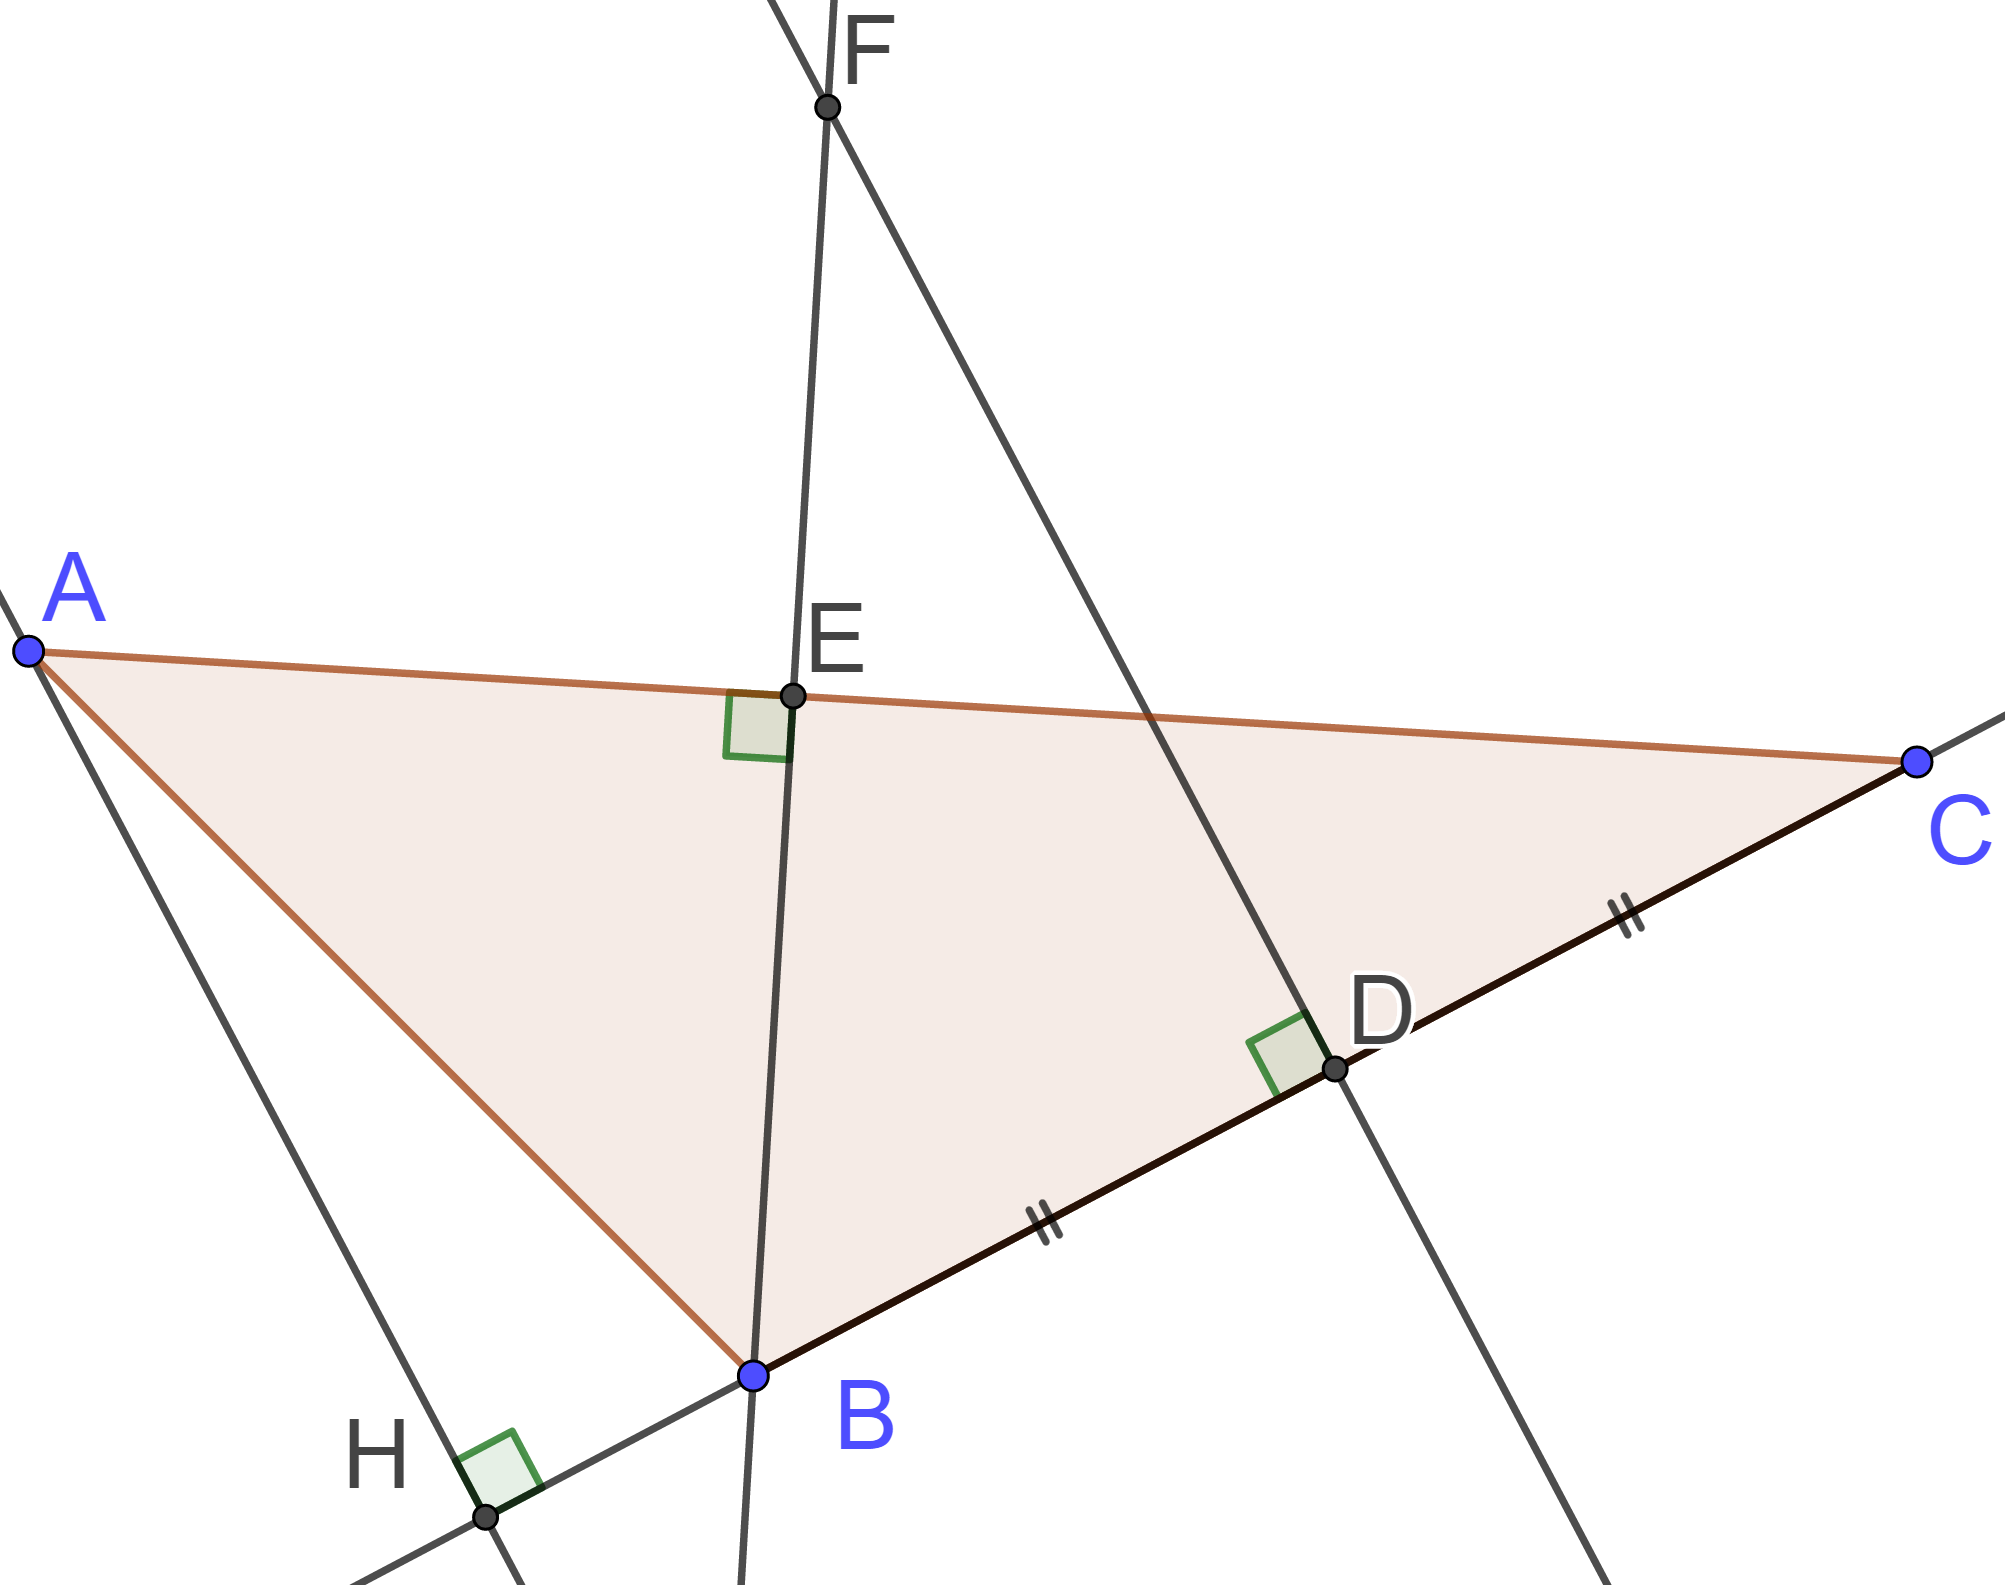
\includegraphics[scale=0.15]{droites}
		\end{center}
	\end{multicols}
\end{myexs}

\section{Les Dalton}

Les tailles des Dalton (en mètres) sont données ci dessous :

\begin{itemize}
	\item $1 + \dfrac{11}{10} + \dfrac{3}{100}$;
	\item $\dfrac{167}{100}$;
	\item $1 + \dfrac{9}{10} + \dfrac{3}{100}$;
	\item Une unité et quatre dixièmes.
\end{itemize}

\begin{questions}
	Retrouve la taille de chaque frère et écris-la sous la forme d'un nombre décimal, en utilisant les informations suivantes :
	
	\begin{itemize}
		\item William et Joe sont plus petits qu'Averell.
		\item Jack est plus grand que William qui est plus grand que Joe.
		\item Averell est plus grand que Jack.
	\end{itemize}
\end{questions}
\label{LastPage}

%\section{Consommation électrique}
%
%Une consommation d'électricité se mesure en 
\end{document}